\documentclass[12pt]{article}
\usepackage[margin=1in]{geometry}
\usepackage{amsmath,amsthm,amssymb,amsfonts}
\usepackage{graphicx}
\usepackage{physics}
%\usepackage{halloweenmath}
\usepackage{setspace}
\usepackage[font=small,labelfont=bf]{caption}

\newcommand{\N}{\mathbb{N}}
\newcommand{\Z}{\mathbb{Z}}

\newenvironment{part}[2][Part]{\begin{trivlist}
\item[\hskip \labelsep {\bfseries #1}\hskip \labelsep {\bfseries #2.}]}{\end{trivlist}}
%If you want to title your bold things something different just make another thing exactly like this but replace "problem" with the name of the thing you want, like theorem or lemma or whatever

\graphicspath{ {./} }

\begin{document}

\title{\textbf{ASTR 522: Problem Set 1}}
\author{Jonas Powell}
\maketitle


%\twocolumn
\begin{onehalfspacing}


\iffalse
You are performing a set of very long baseline interferometric observations using the VLBA, a set of radio telescopes whose longest baseline connects telescopes in Hawaii and St. Croix (19.80159°N 155.45581°W and 17.75652°N 64.58376°W, respectively, according to the wikipedia).
\fi

\iffalse
A) What is the separation, in meters, between these dishes? How well can you know this value? What are the limiting factors on the accuracy with which you can know, and how does this impact the precision with which you can determine the answer? Observations with the VLBA are conducted at GHz frequencies, λ ≈ 10cm.
\fi


\raggedright{\textbf{\Large Problem 1}}\\
\raggedright{\textbf{\large Part A: }}
We would like to begin by finding the spatial separation between the two given dishes. We may first note that, since we are on a sphere, we may consider the distance between the two points in one of two ways: as the (linear) cord connecting the two points, or as the arc along the sphere's surface connecting them. Each of these turns out to be a useful value: the cord-length is used in finding the projected baseline length between the two dishes, while the arc between dishes is necessary to know to calculate the time delay between the two signals, since the information must travel along the Earth's surface. \bigskip

Since we know that both cases rely on the fact that the shortest path between two points on a sphere lies in the Great Circle that contains both points, we realize that what we are really looking for is the angle defined by the two points and the Earth's center. Then we may use that to either calculate the third side of the Iscoceles triangle with radius $r = R_{\oplus}$, or the arc length of that angle with $r = R_{\oplus}$. \bigskip

We may do this by recalling that that angle we are after, the angle formed by the dishes and the Earth's center, is given by:

\begin{align*}
  \Delta \theta &= \cos^{-1} \left( \sin{\phi_1} \sin{\phi_2} + \cos{\phi_1} \cos{\phi_2} \cos{\Delta \lambda} \right)
\end{align*}

where $\phi_i$ is each dish's latitude and $\Delta \lambda$ is the difference between the dishes' longitudes. We may then find the cord- and arc-lengths using familiar geometry:

\begin{align*}
  d_{\text{cord}} &= 2 R_{\oplus} \sin(\frac{\theta}{2}) = 8606058 \text{ meters}\\
  d_{\text{arc}} &= R_{\oplus} \theta = 9445962 \text{ meters}
\end{align*}
\bigskip

These seem to be reasonable numbers, since $d_{\text{cord}}$ agrees with the published baseline length for this pair of dishes for the VLBA on Wikipedia, and we would expect the arc to be a bit longer than the cord. \bigskip

We may approximate the error in this measurement by assuming errors of $\pm 1 \times 10^{-6}$ and propogating the error using:

\begin{align*}
  \sigma &= \sqrt{ \left(\frac{\sigma_{\theta}}{\theta}\right)^2 + \left(\frac{\sigma_{R}}{R_{\oplus}}\right)^2}
\end{align*}

According to the astropy constants module, their uncertainty in the Earth's radius is a round zero, so this simplifies to $\sigma = \frac{\sigma_{\theta}}{\theta}$, leaving us with $\sigma_{\text{arc}} = 63.7$ meters and $\sigma_{\text{cord}} = 58.1$ meters. \bigskip

There are, however, some unconstrained errors. For one, we are not actually propogating error through our calculation of $\theta$ itself, but rather just sticking a value onto it. This is mostly due to lack of understanding. Additionally, we assume a smooth, spherical Earth, which ignores both the Earth's true ellipsoidal form and elevation differences in the locations of the two dishes.\bigskip

To find the uncertainty in the resulting angular resolution, we may say that:

\begin{align*}
  \Delta \theta &= \theta \sigma \\
                &= \frac{\lambda}{D} \sqrt{\frac{\sigma_{\lambda}}{\lambda}^2 + \frac{\sigma_{D}}{D}} \\
\end{align*}
This results in angular resolution uncertainties of $\Delta \lambda/D \approx 1.59 \times 10^{-3}$ radians



\iffalse
B) What is the maximum photon arrival time difference between these two facilities, assuming the photons departed the source simultaneously and the source is sufficiently distant for light rays to be parallel? You may assume that time is accurately kept and synced at both facilities. For the purposes of this problem, you may ignore relativistic corrections.
\fi
\bigskip
\raggedright{\textbf{\large Part B: }}
We calculate the maximum difference in photon arrival time by calculating the length of $d$ in Figure 1 for a source at the horizon for one of the dishes, thus maximizing $d$.\bigskip

From this geometry, we see that, since we have chosen a source at the horizon (i.e. altitude=0 for one of the dishes), then $\phi_1 + \phi_2 = \frac{\pi}{2}$ and $\phi_2 = \frac{\pi}{2} - \frac{\theta}{2}$, so $\phi_1 = \frac{\pi}{2} - \frac{\pi}{2} + \frac{\theta}{2} = \frac{\theta}{2}$. Since we also know the lenght of $B$ from part A, then we may find that $d = B \cos{\frac{\theta}{2}} = 6352402$ meters. Multiplying this distance by $c$, we find that the induced time delay is $\Delta t = 0.02$ seconds. Pretty significant!



\iffalse
C) Besides observations of millisecond pulsars, can you think of any astronomical phenomena whose observation would need to be corrected by your previous answers to this problem? For all answers, if you have multiple sources of uncertainty, you may assume that they are small and of similar magnitude, so uncertainties may be combined linearly.
\fi
\bigskip
\bigskip
\raggedright{\textbf{\large Part C: }}
LIGO would probably run into this problem since the frequency of the gravitational waves that it is looking for are higher than this.

\bigskip
\bigskip









\iffalse
Barycenter correction is tricky business and there are a lot of factors that go into it. To see a modern application, please review this paper: Wright & Eastman, 2014 PASP, 126 838. http://adsabs.harvard.edu/abs/2014PASP..126..838W

The authors have provided an IDL code to perform the calculations, along with web applets to interface it. Further folks have provided a Python script to access the web applets. How’s that for abstraction. The Python code is here: https://github.com/tronsgaard/barycorr

Yikes! Let’s start with a simpler task, but we’ll keep this in mind for later. The Hubble Space Telescope orbits the Earth in a nearly circular orbit, with altitude of 540 km, and an orbital period of 95 minutes 28 seconds.
\fi

\iffalse
A) If left unchecked, how much would Hubble’s clock become out of sync in one year, compared to a clock at sea level? Assume that time is kept by identical atomic clocks onboard Hubble and on the ground, and that their systematic errors are negligible.
\fi

\raggedright{\textbf{\Large Problem 2}}\\
\raggedright{\textbf{\large Part A: }}

As in Monday's class, we may solve this problem by calculating and combining contributions from Special and General Relativity.

\bigskip

\textbf{Special Relativistic Effects:}
\begin{align*}
  \gamma^{-1} &= - \frac{v^2}{2 c^2} \times 3.1536 \times 10^7 \text{seconds year$^{-1}$}\\
              &= 0.0101 \text{ seconds year$^{-1}$}\\
\end{align*}


\textbf{General Relativistic Effects:}
\begin{align*}
  \Delta \gamma^{-1} &= \frac{G M_{\oplus}}{c^2} \times \left( \frac{1}{R_{\oplus}} - \frac{1}{R_{\text{Satellite Orbit}}} \right)  \times 3.1536 \times 10^7 \text{seconds year$^{-1}$}\\
                     &= -0.0017  \text{ seconds year$^{-1}$} \\
\end{align*}


Summing these two, we find that over a year, the Hubble's clock would drift back by 0.00839 seconds, or about 8.4 milliseconds, over the course of the year.






\iffalse
B) Let’s consider part B from problem 1 in the context of a moving satellite compared with the Keck telescope on Mauna Kea. Our baseline is now constantly changing! Thankfully we’re no longer doing interferometry! What is the maximum photon arrival time difference between these two facilities? What’s the time difference an hour (at Mauna Kea) later? How does your answer compare with the answer to part A?
\fi
\bigskip
\bigskip

\raggedright{\textbf{\large Part B: }}
In this case, we may maximize the difference in photon arrival time by observing a source at zenith over Mauna Kea and seeing how far around the Earth we can send the satellite before it can no longer see the source (see Figure 2). If the satellite's altitude was zero, then a quarter circle would be the farthest we could wrap around, but since it has some altitude, it is able to go a little bit further around the Earth and still catch the signal. Therefore, it is at this point that the photons from the source have the largest relative difference in path length, and consequently the largest time difference as well. \bigskip

The important quantity we want, then, is the leg of the triangle connecting the satellite to the surface of the Earth, in line with the light from the source. Since we know the triangle's other two legs ($R_{\oplus}$ and $R_{\oplus} + H_{\text{Satellite Orbit}}$), then we can easily find the third leg's length as well.

\begin{align*}
  d &= \sqrt{(R_{\oplus} + H)^2 - R_{\oplus}^2} \\
    &= 9.409580 \times 10^6 \text{ meters} \\
  \rightarrow d_{\text{Total}} &= d + R_{\oplus} \\
                   &= 1.42\, R_{\oplus} \\
  \rightarrow \Delta t &= \frac{d}{c} = 0.03 \text{ seconds}
\end{align*}

In this configuration, light would reach Mauna Kea 0.03 seconds before reaching Hubble. \bigskip

Allowing things to progress an hour makes this a bit of a trigonometric nightmare.

We begin by defining some values we will find useful:
\begin{align*}
  R &= R_{\oplus}\\
  \text{alt} &= \text{Altitude of Mauna Kea observatory (meters above sea level)} \\
  H &= \text{HST Orbital Height} \\
  l &= \text{Cord length between HST and Keck}\\
  \theta_{\text{HST}} &= \text{Angular change of HST in 1 hour} \\
\end{align*}

This is now a harder problem to solve since we can no longer lean on the right triangle that we had in the previous problem, so while in principle the problem is still just one of finding the projected distance between the observatories along the path of the source's light, it becomes a lot messier, quite quickly. \bigskip

We begin by considering the triangle defined by the line connecting the center of the Earth with the Mauna Kea observatory ($r = R_{\oplus} + \text{alt}$), the line connecting the center of the Earth and HST ($r = R_{\oplus} + H$), and the line connecting HST and Mauna Kea. We define $\theta_i$ to be the angle defined by Mauna Kea, the center of the Earth, and HST, and we define $\alpha$ to be the angle defined by the center of the Earth, HST, and Mauna Kea. We would now like to find expressions for how long the cord $l$ connecting the two observatories is, as well as an angle we will call $\theta$, the portion of $\alpha$ that extends past the plane perpendicular to the incoming light wave (see Figure 3). \bigskip


As we can now easily see, the quantity we want is $d$, since that is the difference in the path length between photons hitting each observatory. Simple trigonometry tells us $d = l \, cos{\theta}$. Our task now is to solve for $l$ and $\theta$.

\bigskip
\bigskip


\begin{figure}

\end{figure}

We solve for $l$ using the geometry shown in Figure 4 by using the fact that we know $\theta_i$ to find the base of the left-side right triangle defined along the the line connecting the center of the Earth and HST. With that in hand, we can easily find the right-side right triangle along the same line, and thus find an expression for $l$ as a function of $\alpha$ and $\theta_i$. This yields:
\begin{align*}
  l &= \frac{R + H - (R + \text{alt}) \cos \theta_i}{\cos \alpha} \\
\end{align*}

We may find $\theta$ using the Law of Sines and plugging in our expression for $l$:
\begin{align*}
  \frac{l}{\sin(\theta_i)} &= \frac{R + \text{alt}}{\sin \alpha} \\
  \frac{R + H - (R + \text{alt}) \cos{\theta_i}}{\cos \alpha \,\, \sin \theta_i} &= \frac{R + \text{alt}}{\sin \alpha} \\
  %\rightarrow \alpha &= \sin^{-1} \left( \frac{R + \text{alt}}{l} \, \sin(\theta_i) \right) \\
  %\rightarrow \theta &= \alpha - \left( \frac{\pi}{2} - \theta_{\text{sat}} \right) \\
\end{align*}

Rearranging, we find:

\begin{align*}
  \tan \alpha &= \frac{ (R + \text{alt}) \sin \theta_i}{R + H - (R + \text{alt}) \cos \theta_i} \\
  \alpha &= \tan^{-1} \left( \frac{ (R + \text{alt}) \sin \theta_i}{R + H - (R + \text{alt}) \cos \theta_i} \right) \\
\end{align*}

Again referring to Figure 3, we notice that we have a right triangle defined by the angles $\theta_{\text{HST}}, \alpha - \theta$, and $\pi/2$. Therefore, we find $\pi = \pi/2 + (\alpha - \theta) + \theta_{\text{HST}}$, so $\theta = \alpha + \theta_{\text{HST}} - \pi/2$.


Combining our expressions for $\theta$ and $l$, we may finally find the distance $d$ that we have been looking for:


\begin{align*}
  d &= l \,\, \sin \left( \tan^{-1} \left(   \frac{R \, \sin(\theta_i)}{R + H - (R + \text{alt}) \cos{\theta_i}} \right) - \frac{\pi}{2} + \theta_{\text{HST}} \right) \\
  \rightarrow \Delta t (\theta_i, \alpha, H, \text{alt}, t) &= \frac{d}{c} \\
                       &= \frac{l}{c} \,\, \sin \left( \tan^{-1} \left(   \frac{R \, \sin(\theta_i)}{R + H - (R + \text{alt}) \cos{\theta_i}} \right) - \frac{\pi}{2} + \theta_{\text{HST}} \right) \\
\end{align*}

Hurrah! Even though that's an awful-looking equation, it's extremely solvable, so we just need to plug in our values (note that I think the equation is a lot clearer in code than here; see Python file attached). We already know that $R = R_{\oplus}$ and $\text{H} = 5.4 \times 10^5$ meters, and a quick Google search reveals that Mauna Kea's elevation is $\text{alt}=4205$ meters.

\bigskip
\bigskip

We find $\theta_i$ by summing the angles that each of the observatories makes with the direction that the light is coming in at, i.e. $\theta_i = \theta_{\text{HST}} + \theta_{\text{MK}}$. $\theta_{\text{MK}}$ is trivial; it is simply $\theta_{\text{MK}} = \frac{2 \pi (1 \text{ hour})}{24 \text{ hours}} = 0.2618$ radians. $\theta_{\text{HST}}$ is a little harder to find. Using the geometry described by Figure 4, we may find it by recognizing that it is the fraction of the circle left over when the first quadrant of the circle, the angular offset found  earlier for HST's initial position, and the change in angular position over the course of the hour are all subtracted from $2 \pi$. In other words,
\begin{align*}
  \theta_{\text{HST}} &= 2 \pi - \left(\frac{\pi}{2} + \sin^{-1} \left( \frac{R}{R + H}\right) + \frac{2 \pi (1 \text{ hour})}{1.591 \text{ hours}} \right) \\
                      &= 0.365 \text{ radians} \\
\end{align*}

and therefore $\theta_i = 0.3654 + 0.2618 = 0.6272$ radians. Plugging all these values in gives us a final difference in path length of -0.05 $R_{\oplus}$, corresponding to a difference in photon arrival time of -0.986 milliseconds. These numbers make sense: we expect the differences to be much smaller than the maximum difference that we calculated earlier, since HST travels a signficant portion of its orbit in an hour, meaning that it is on the "front" of the Earth by the time this second measurement is taken. The negative sign reflects the fact that the light from the source is actually reaching HST before it reaches Mauna Kea, which again makes sense for the same reason.










%% FIGURES
\newpage


%\iffalse
\begin{figure}
    \centering
    \begin{minipage}{0.48\textwidth}
        \centering
        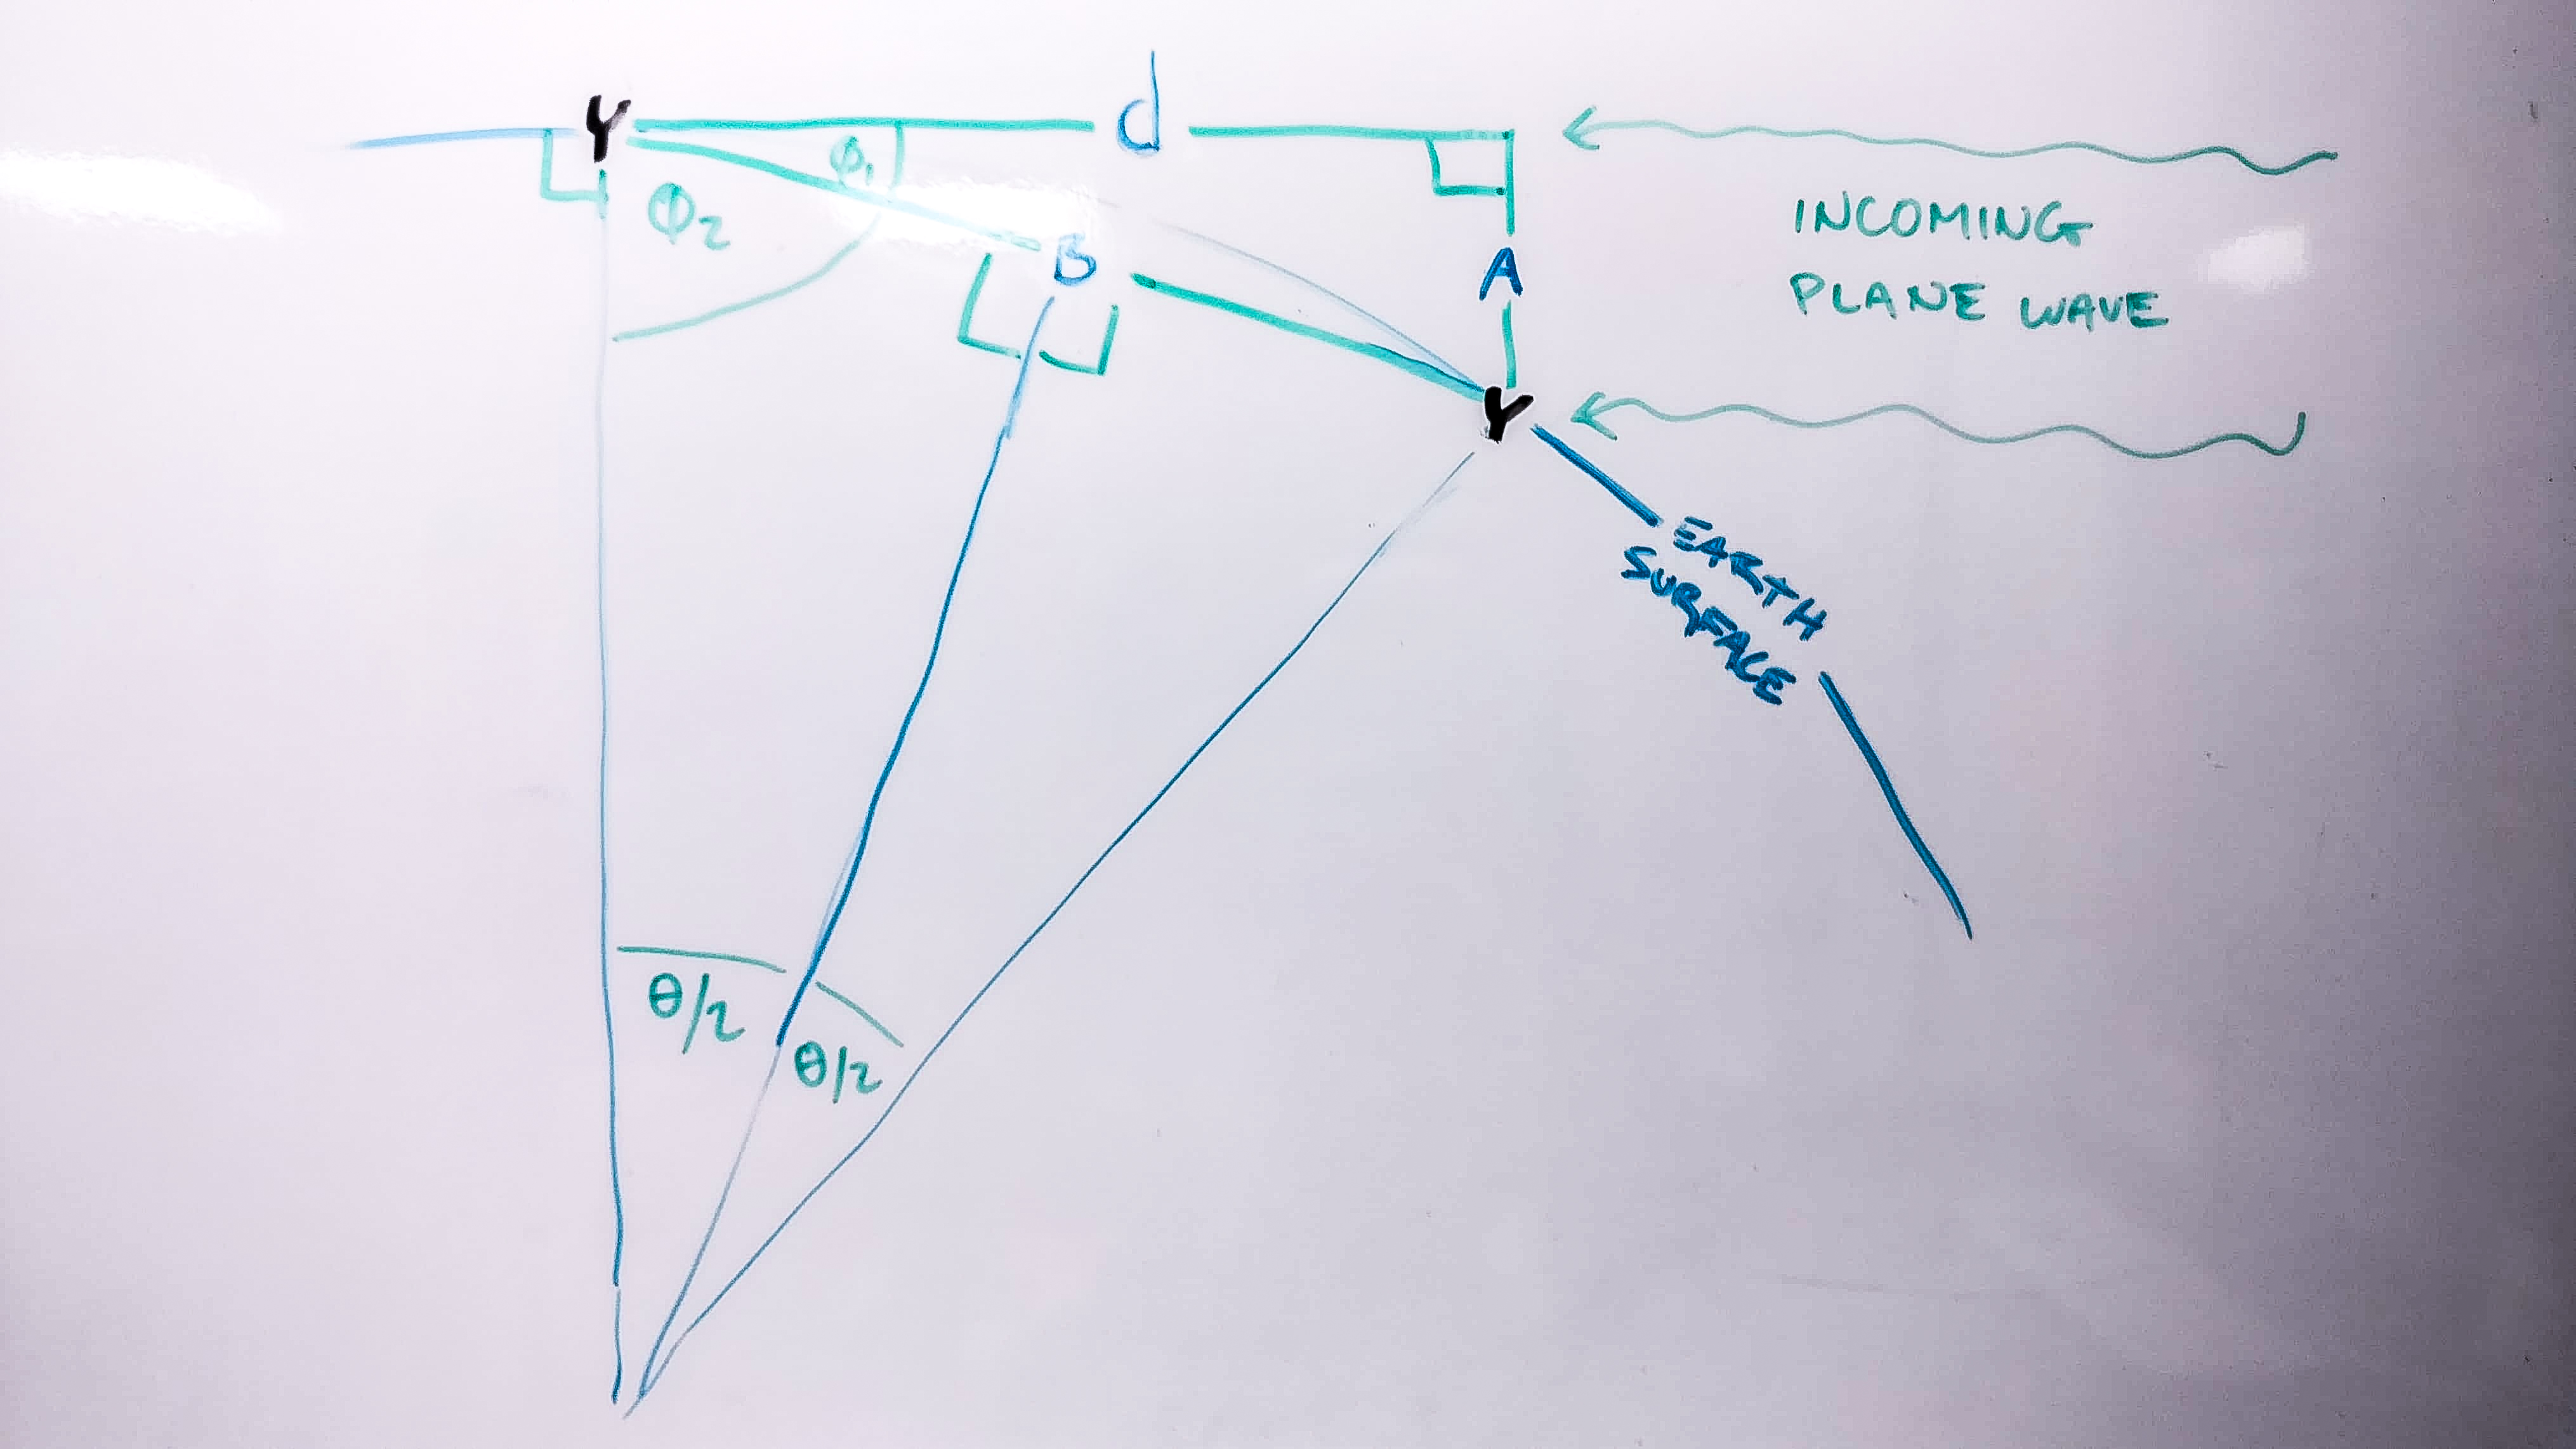
\includegraphics[width=0.95\textwidth]{prob1b} % first figure itself
        \caption{Signal from a source at one source's horizon results in this geometric event, from which we can find difference in path length for signal reaching each dish.}
    \end{minipage}\hfill
    \begin{minipage}{0.48\textwidth}
        \centering
        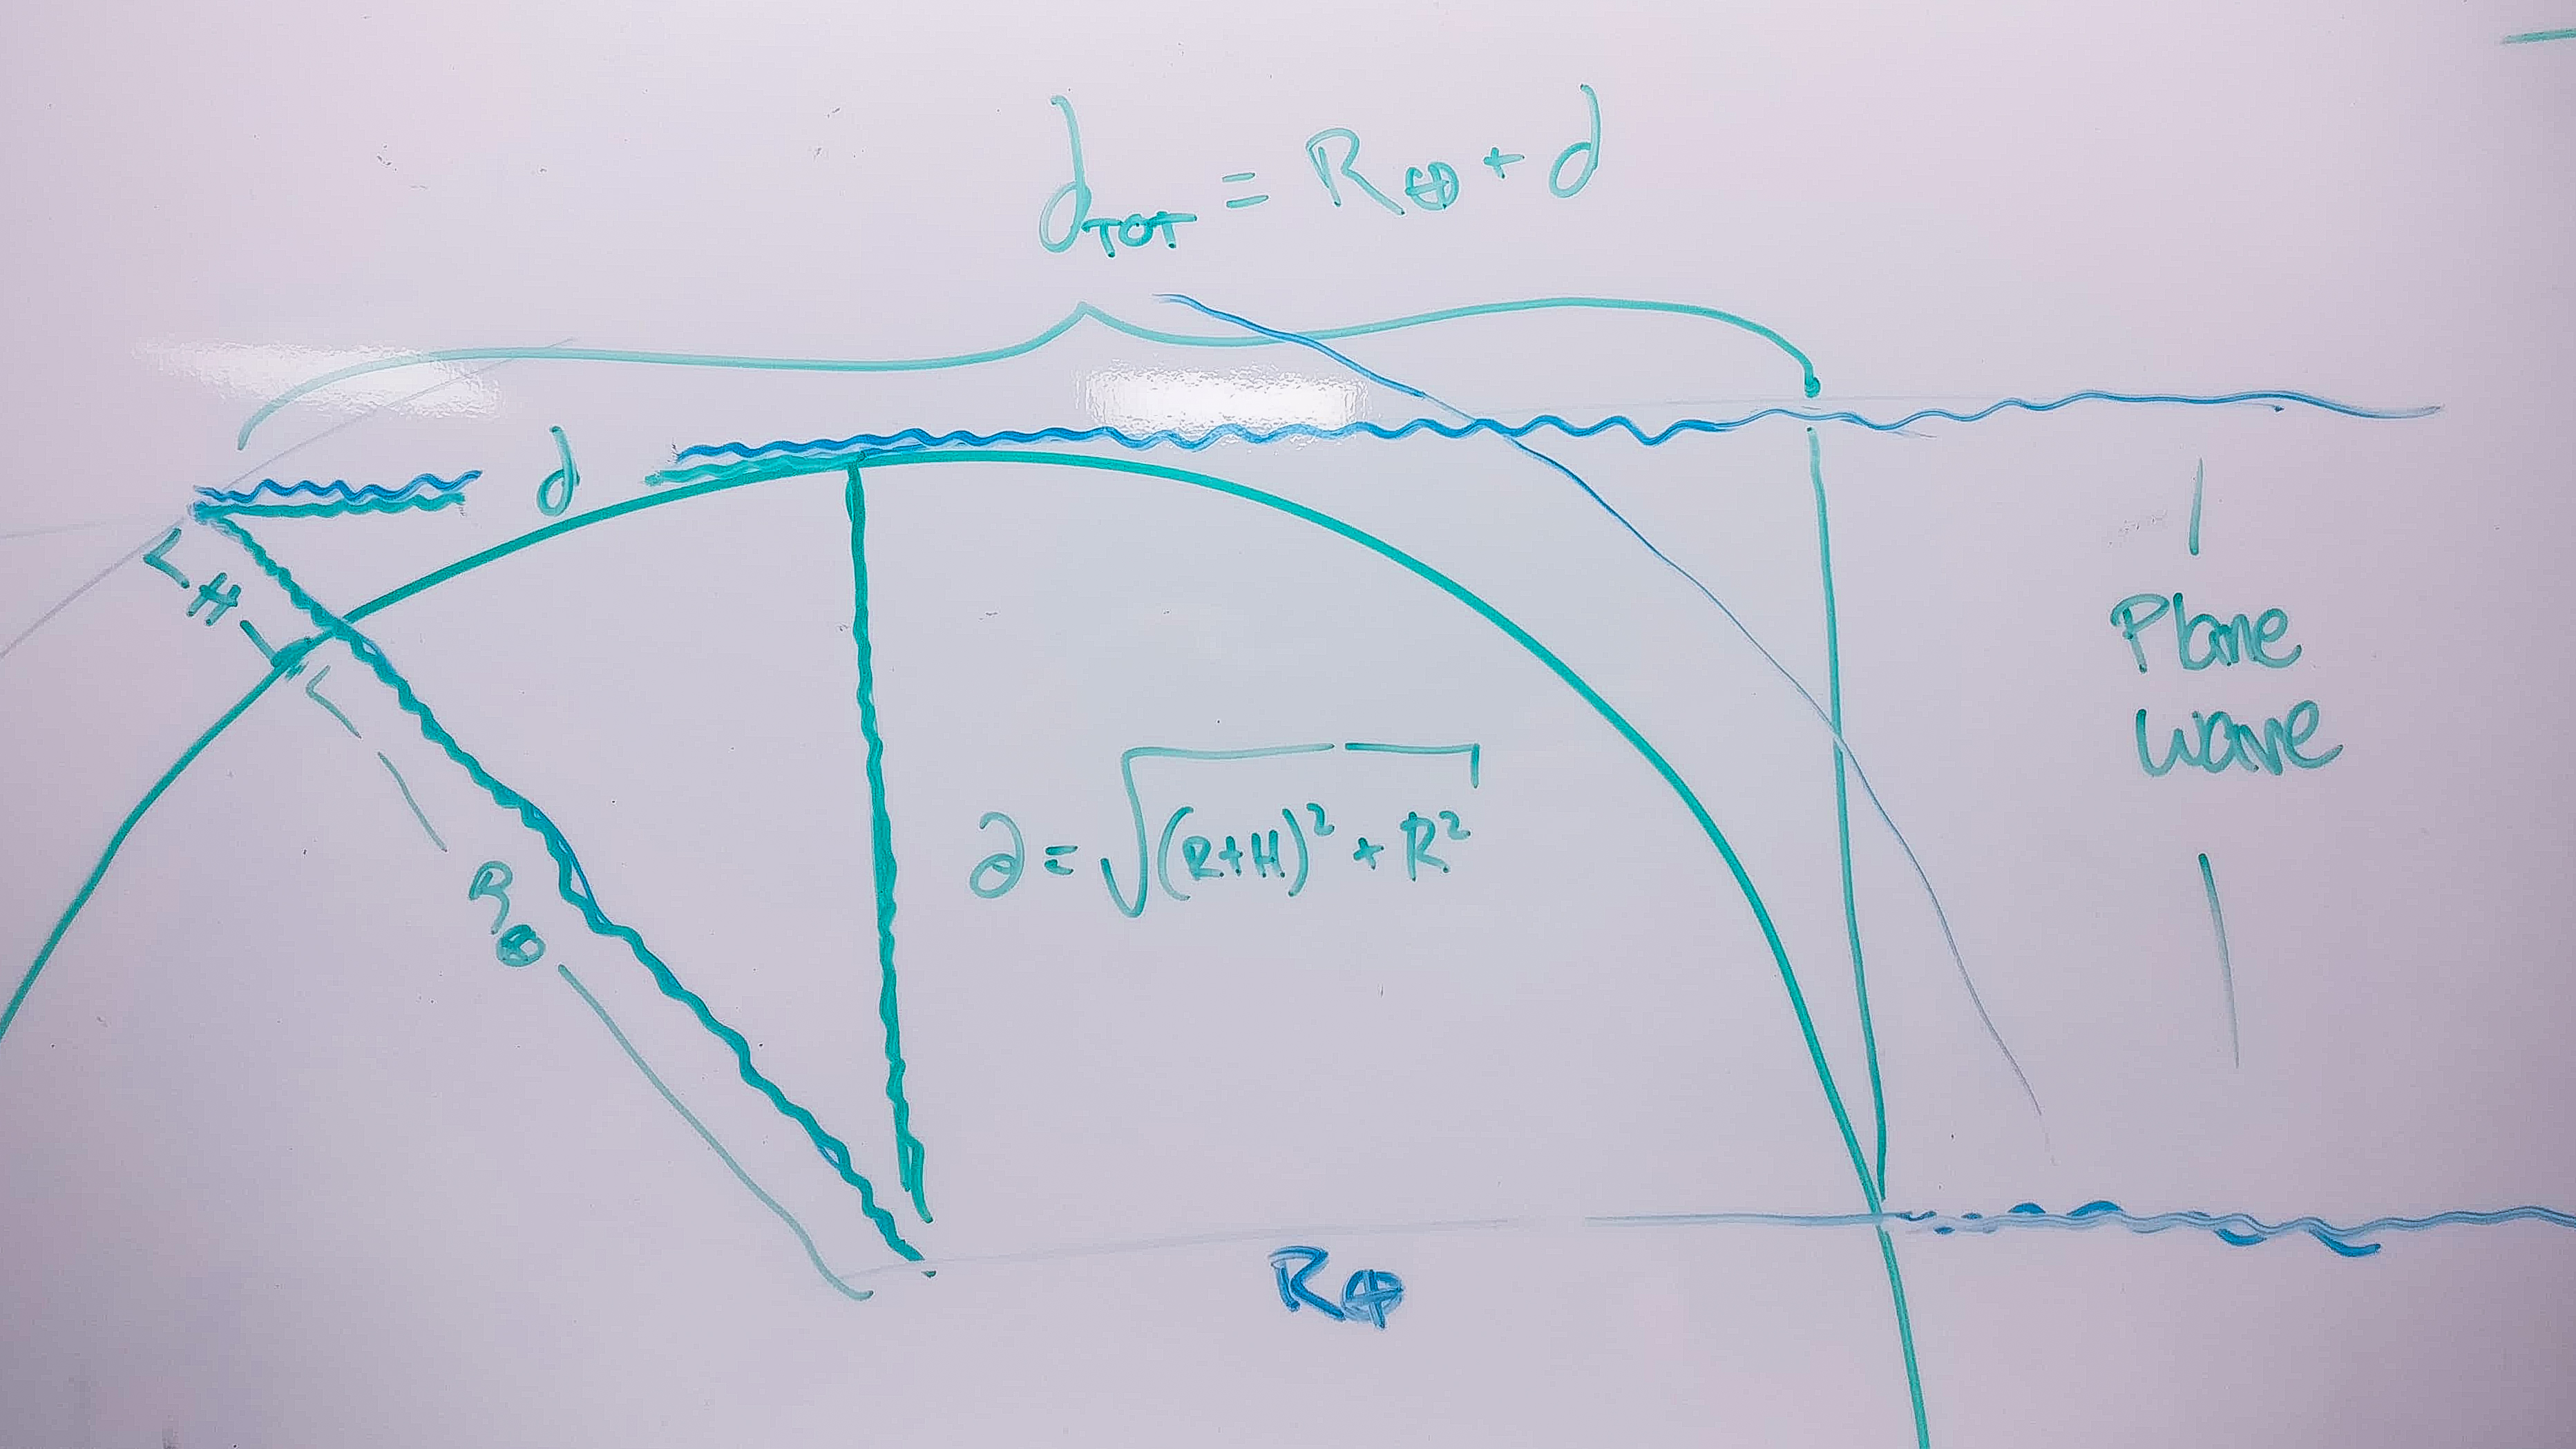
\includegraphics[width=0.95\textwidth]{prob2b} % second figure itself
        \caption{Signal from a source at one source's horizon results in this geometric event, from which we can find difference in path length for signal reaching each dish.}
    \end{minipage}
\end{figure}

\begin{figure}
    \centering
    \begin{minipage}{0.48\textwidth}
        \centering
        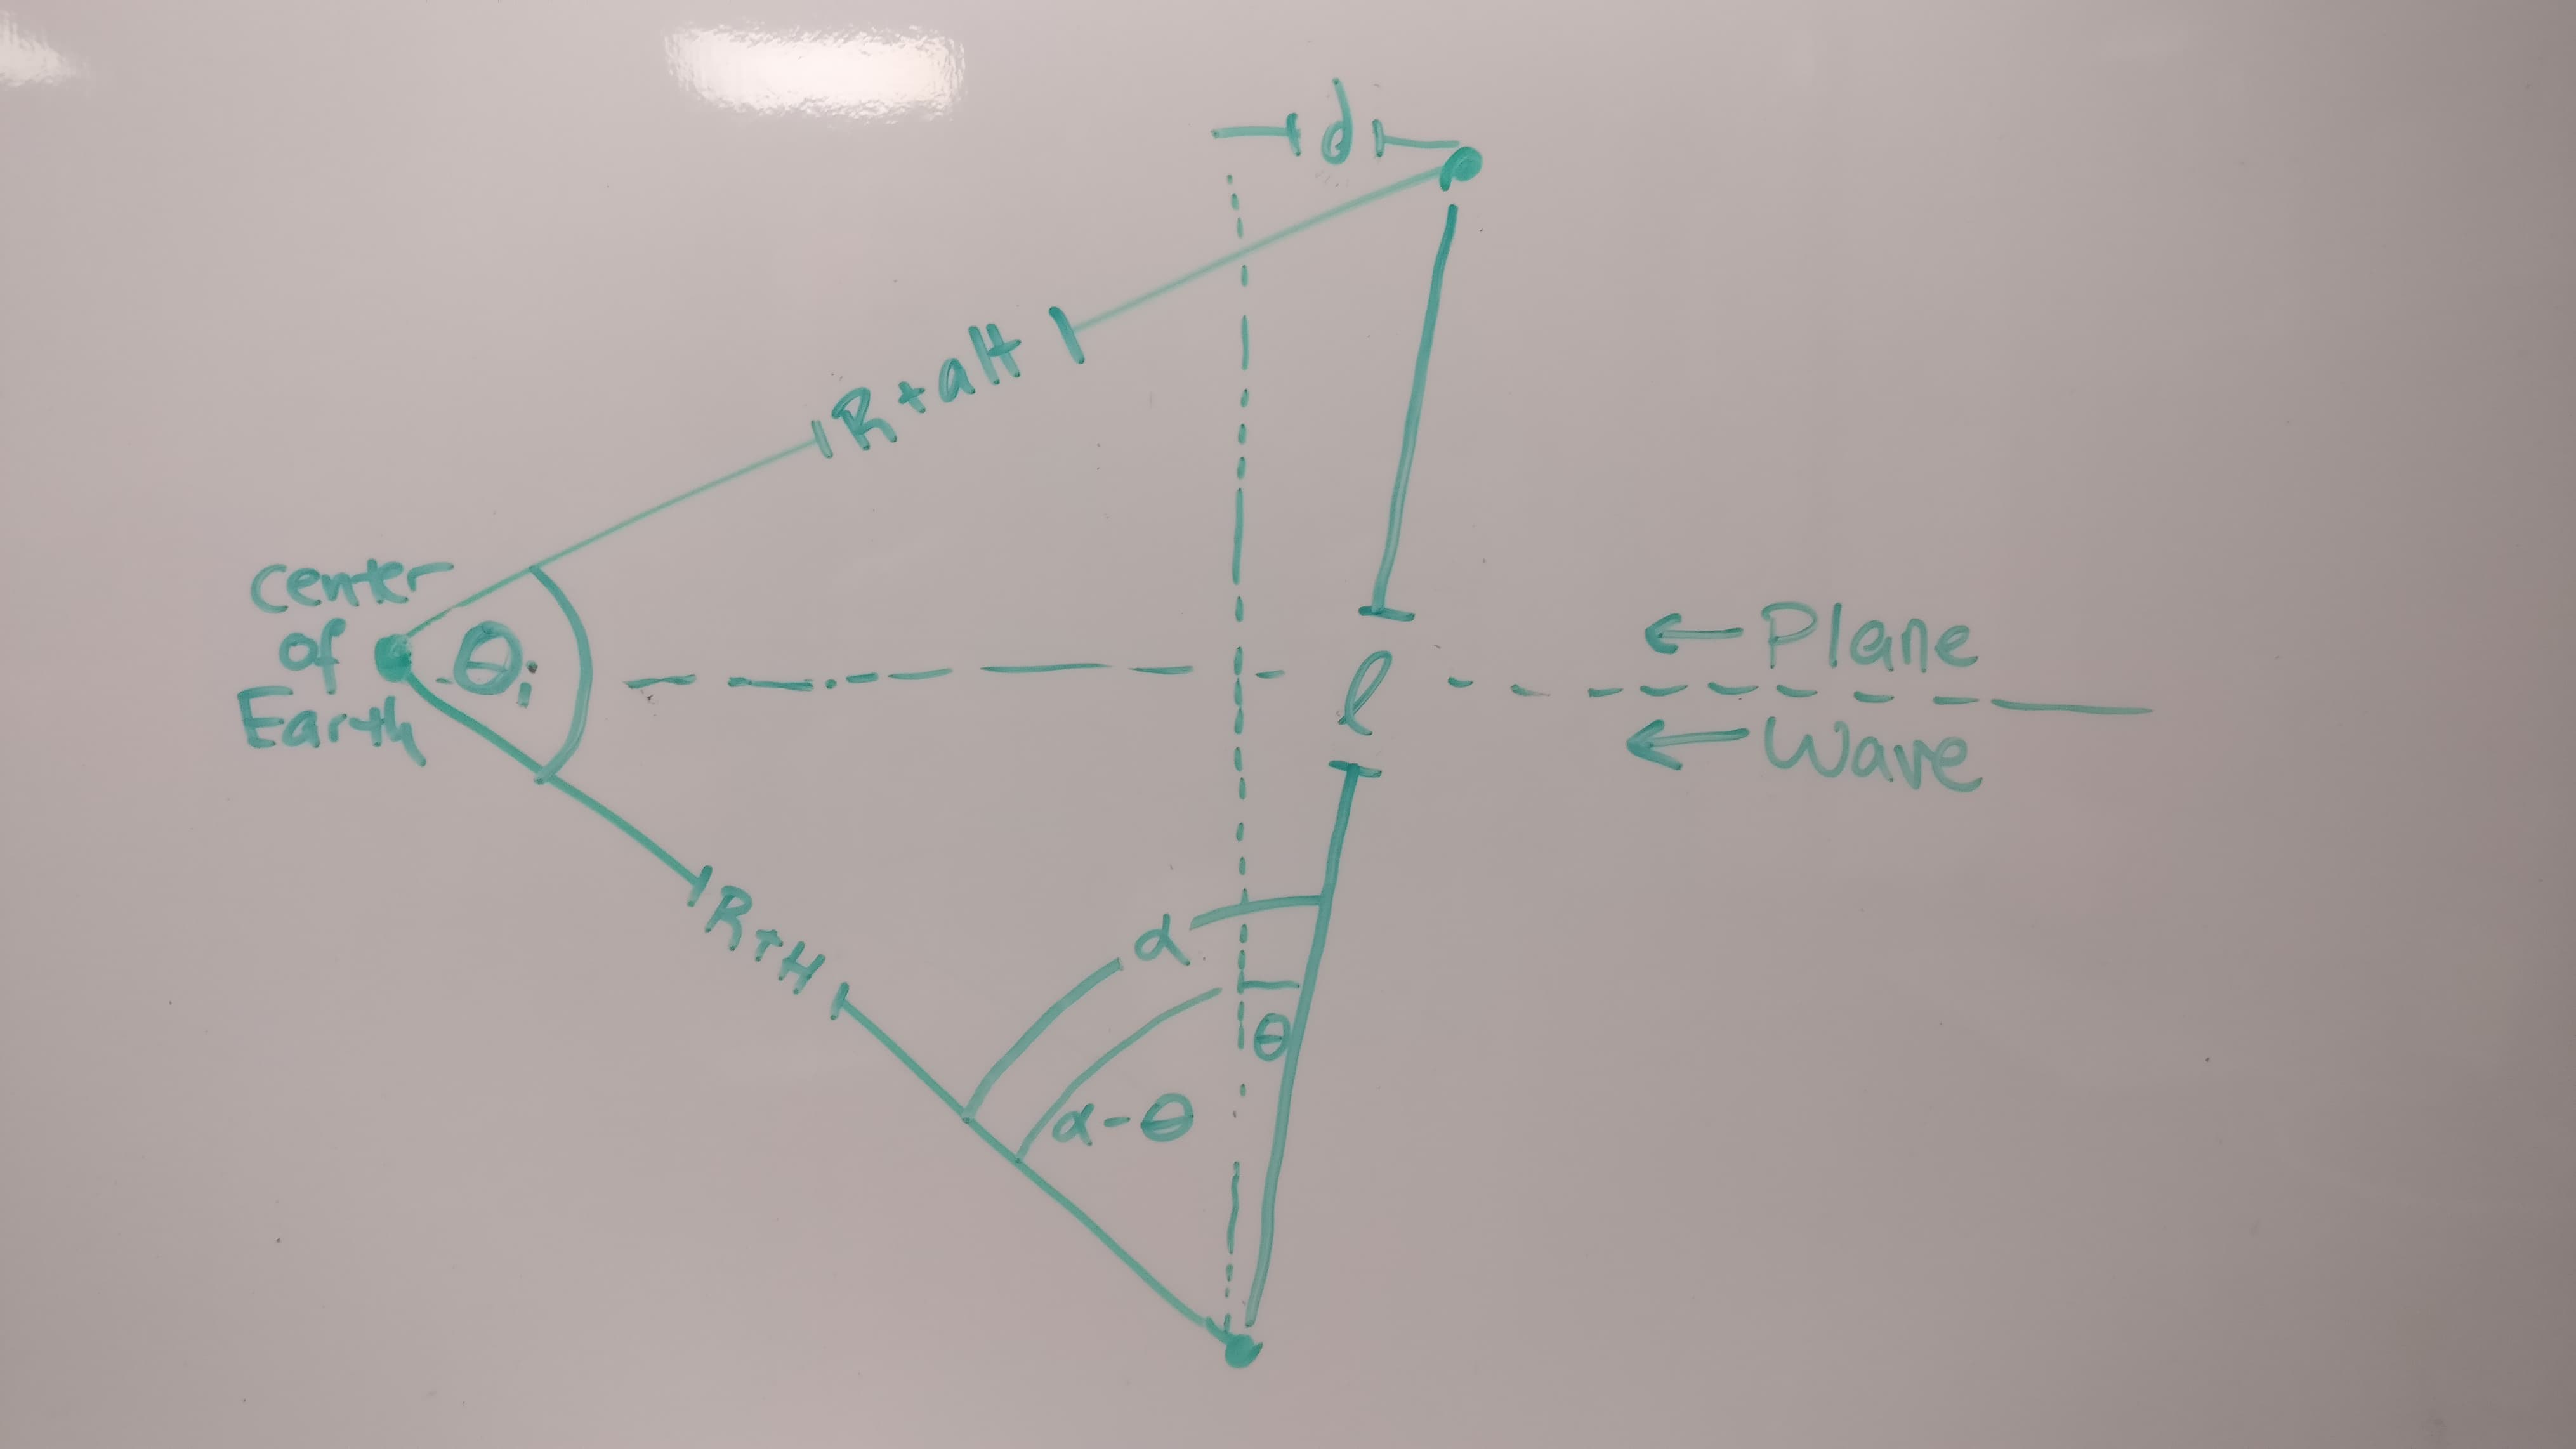
\includegraphics[width=0.95\textwidth]{prob2b-1} % first figure itself
        \caption{Establishing the geometry we will use.}
    \end{minipage}\hfill
    \begin{minipage}{0.48\textwidth}
        \centering
        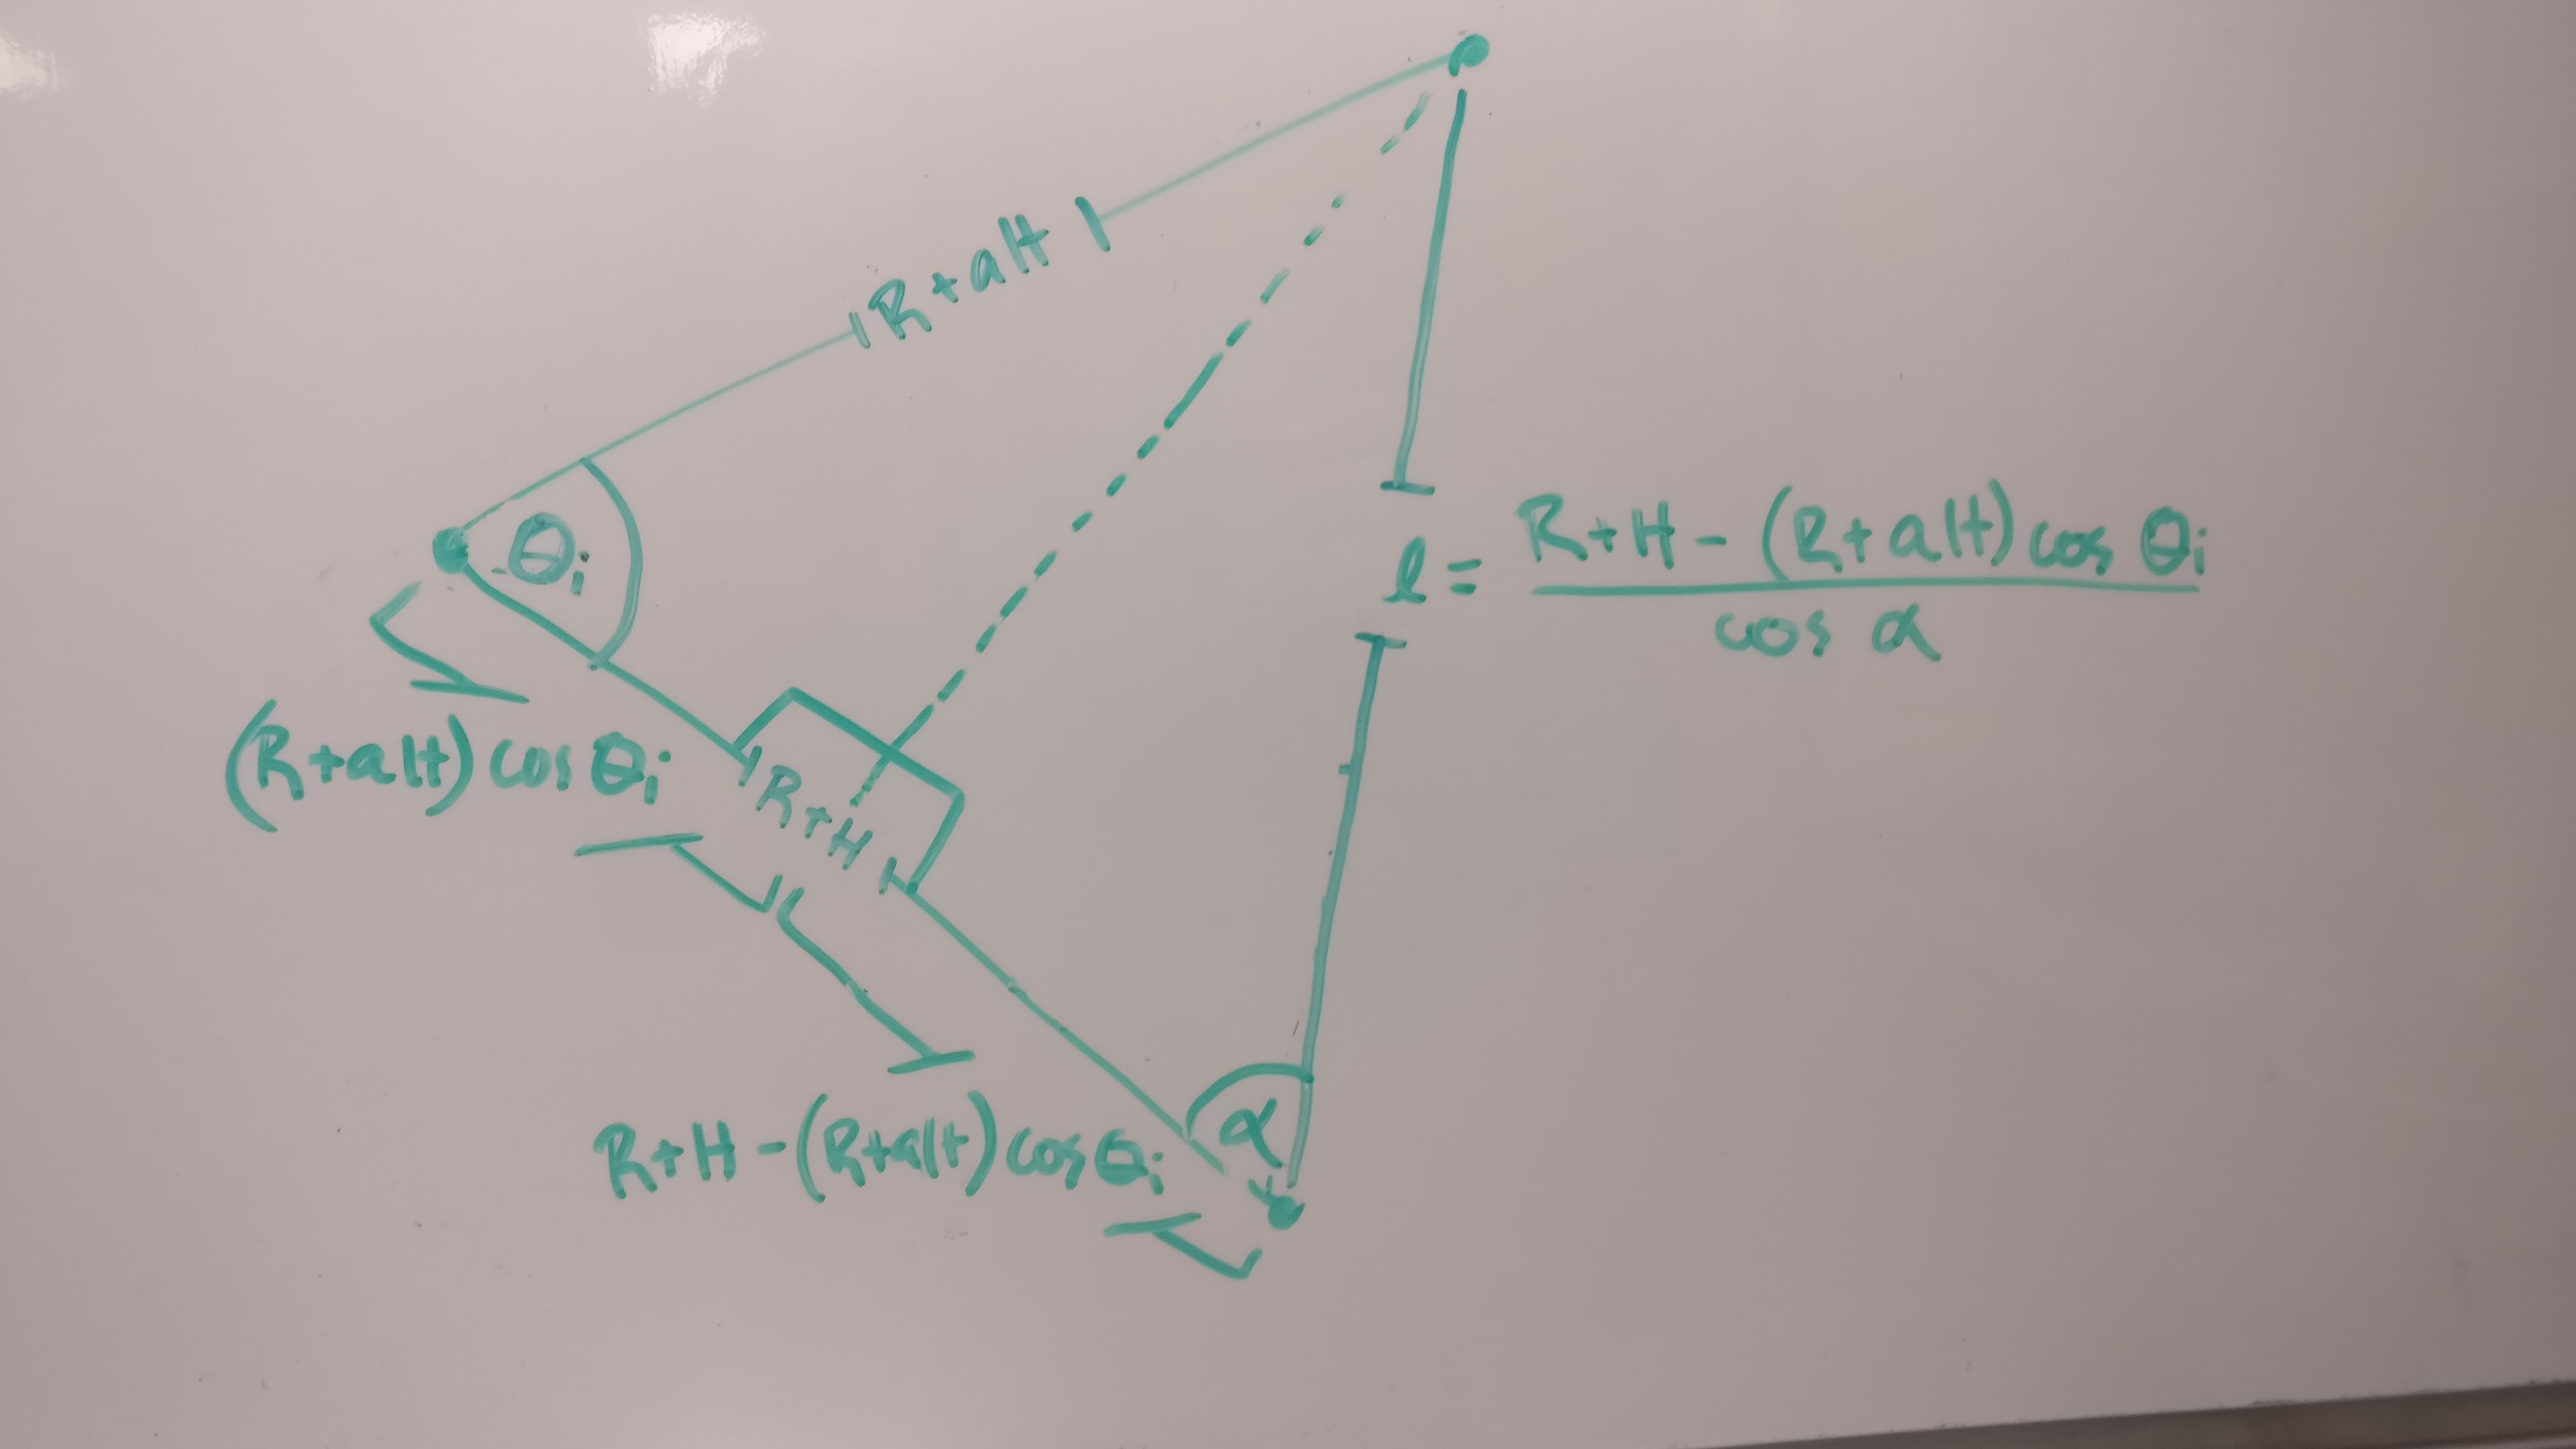
\includegraphics[width=0.95\textwidth]{prob2b-2} % second figure itself
        \caption{Finding $l$.}
    \end{minipage}
\end{figure}

\begin{figure}
    \centering
    \begin{minipage}{0.48\textwidth}
        \centering
        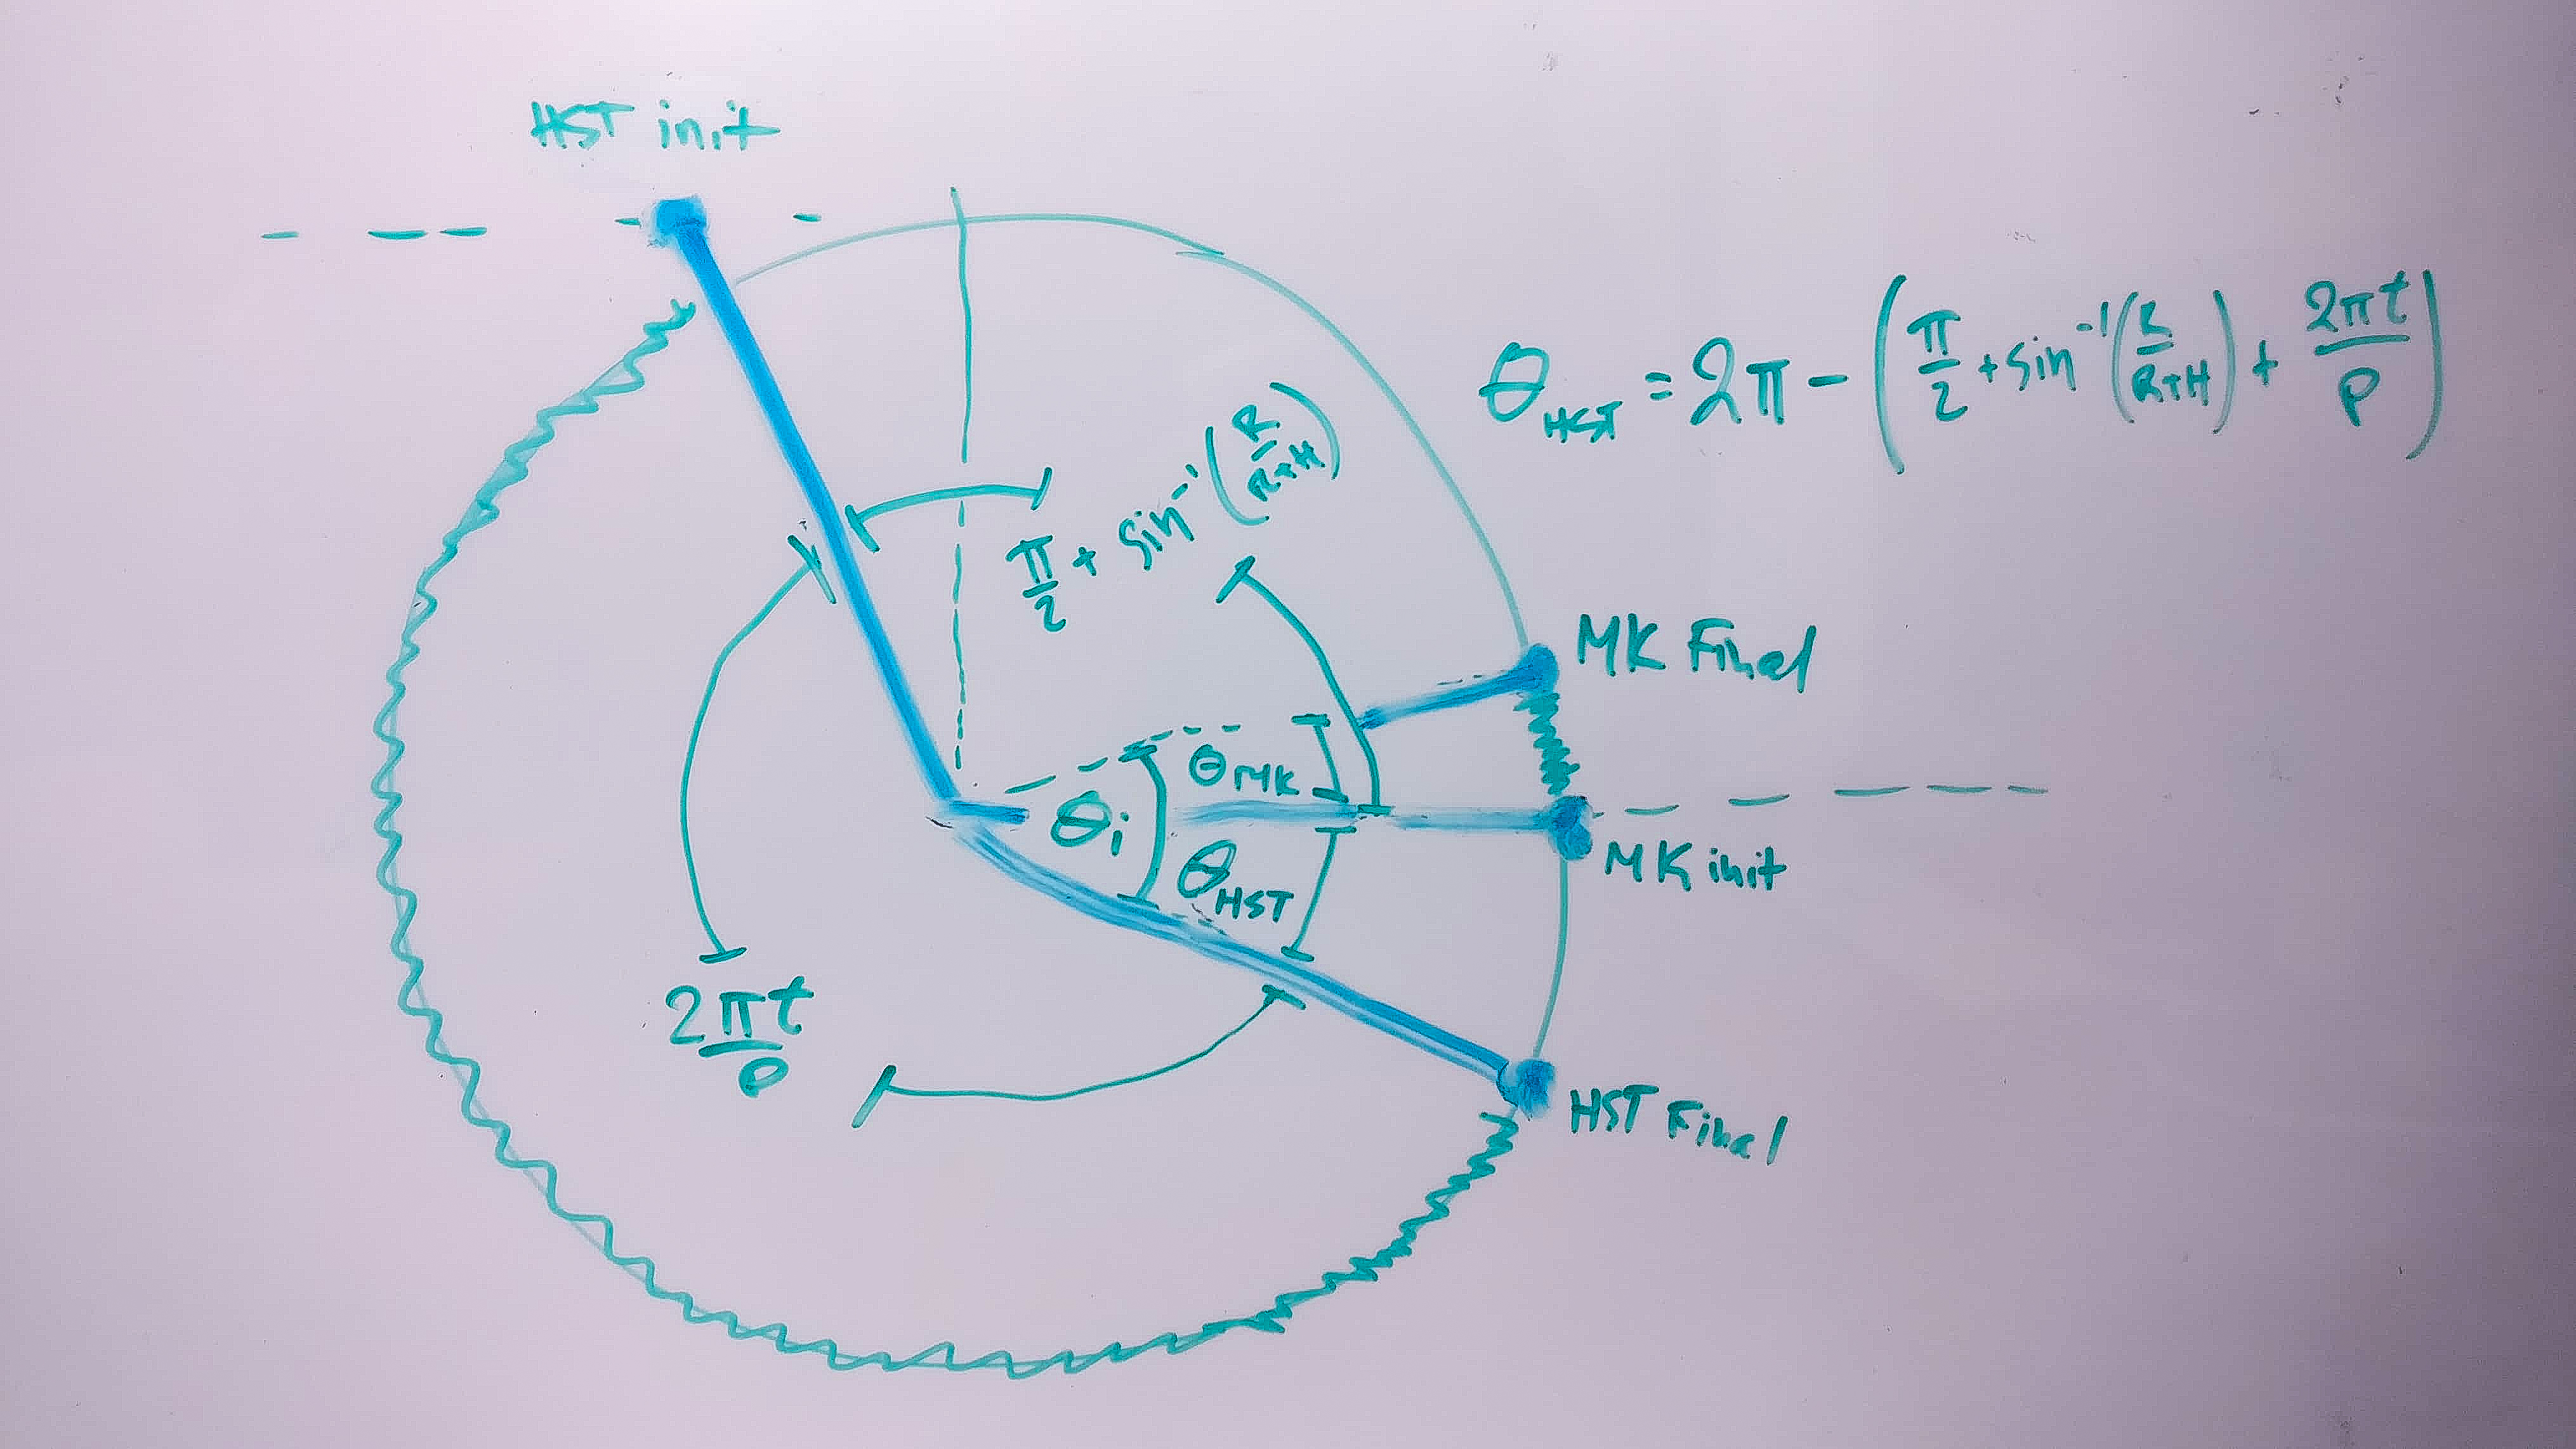
\includegraphics[width=0.95\textwidth]{prob2b-3} % second figure itself
        \caption{Finding $\theta_i$.}
    \end{minipage}
\end{figure}
%\fi






\bigskip
\bigskip
\end{onehalfspacing}

\end{document}
